\documentclass[a4paper,utf8,10pt]{article}
\usepackage[UTF8]{ctex}
\usepackage{geometry, fontspec, fancyhdr, scalefnt, minted, caption, cite, wrapfig, graphicx, tikz, tikz-network, float, amsmath, amssymb}
\usepackage[pdfauthor={梁亚伦, 吴轩南, 李信义; 指导教师: 卢婧华, 武迪},
            pdftitle={基于LSTM的视频配乐智能分类系统的研究与开发},
            pdfsubject={中国人民大学附属中学研究性学习, 2020年},
            pdfkeywords={情绪识别;音频分类;视频配乐}]{hyperref}
\usepackage[affil-it]{authblk}

\geometry{a4paper, top=2cm, left=1.5cm, bottom=1.8cm, right=1.4cm}
\setlength{\headheight}{0pt}
\fancypagestyle{plain}{
  \fancyhf{}
  \renewcommand{\headrulewidth}{0pt}
  \renewcommand{\footrulewidth}{0pt}
}
\pagestyle{empty}
\linespread{1.56}
\scalefont{1.05}

\newcommand{\sept}{\setlength\itemsep{-4pt}}
\newcommand{\somefigure}[4]{
  \begin{figure}[#4]
    \begin{center}
      \vspace{-13pt}
      \includegraphics[width=0.8\textwidth]{#1}
      \vspace{-10pt}
      \caption{#2}
      \label{#3}
      \vspace{-10pt}
    \end{center}
  \end{figure}
}

\title{基于 LSTM 的视频配乐智能分类系统的研究与开发}
\author{梁亚伦  吴轩南  李信义 \\ 指导教师: 卢婧华  武迪}
\affil{中国人民大学附属中学  北京  100080}
% \date{2020年5月29日}
\date{}

\begin{document}

\maketitle

\begin{abstract}
目前市面上常见的视频配乐软件曲库简单,情绪、流派等分类单一,已有的音乐特征识别软件虽然相对成熟,但还没有开发者尝试将音乐特征识别应用于视频配乐分类。
本文所做研究希望制作一个智能配乐分类系统,自动识别曲库中所有音乐的情绪、流派等信息,帮助视频制作者提高配乐选取效率。
本文首先完善通过爬虫方式获得的训练材料并设计音乐分类体系,之后提取音乐特征用于训练。在训练环节,本文首先尝试传统的 $k$-近邻和支持向量机算法,
但都出现维度灾难、无时序性等问题。最终,研究选取 LSTM 算法进行训练并封装程序,效果比较符合预期。
本文中所选取的 LSTM 算法在情绪、基调等特征的识别准确率大致达到了 75.4\%、85.5\%,但乐器识别由于标签过于混乱导致效果仍有待改进。
后期可以完善的方向包括寻找更好的数据源完善乐器识别功能、尝试使用自相似矩阵等其他音乐特征、使用其他神经网络进行实验进一步提升识别的准确率等。
\end{abstract}

\paragraph{关键词} 情绪识别、音频分类、视频配乐
%\vspace{\baselineskip}

\section{引言}

\subsection{研究背景及意义}

随着视频社交网络的普及,剪辑微电影、Vlog 剪辑逐渐成为人们记录生活的途径。市面上流行的视频制作软件主要专注于视频剪辑和特效,
在配乐方面通常曲库都比较简单,情绪和乐器上种类也比较单一~\cite{boixx14}。如果制作者想使用自己的音乐,又要花费很多的时间在从众多歌曲中挑选自己心仪的音乐上。
本研究尝试制作一个智能音乐分类系统,可以自动识别曲库中所有音乐的乐器、情绪、时长等信息,
识别成功后制作者可以在搜索框通过搜索所需音乐的特征来对音乐进行筛选,从而更快的找到适合的视频配乐。

\subsection{研究过程}

参见表~\ref{tab:process}。

\begin{table}[h]
\caption{研究过程} \label{tab:process}
\noindent\begin{tabular}{ r | l | p{13.5cm} }
\hline
序号 & 课题阶段         & 具体内容                                                                                     \\ \hline
   1 & 配乐理论知识学习 & 了解电影/视频配乐的历史和传统分类,并根据现实中的需求加入专门针对当下视频制作者的分类。      \\ \hline
   2 & 设计音乐分类体系 & 基于 YouTube Audio Library~\cite{yal} 上对音乐分类的标签进行去重、调整和添加,整理出后期用于分类的音乐分类体系。\\ \hline
   3 & 准备训练资料     & 编写爬虫程序,从 YouTube Audio Library 上下载用于训练的音频文件和标签,通过人工核查整理的方式完善标签,包括合并重复或意思相同的标签、去除明显错误的标签等。                    \\ \hline
   4 & 提取关键信息     & 通过 LibROSA~\cite{librosa18}~从音乐中提取特征,判断挑出其中对训练模型有用的特征,量化之后作为训练所需要的数据。           \\ \hline
   5 & 初步进行训练     & 选取适当准确的模型,找出各个音乐元素与最终分类之间的关联。                                   \\ \hline
   6 & 形成分类系统     & 形成适合于视频配乐的音乐分类系统。                                                           \\ \hline
   7 & 算法的完善优化   & 尝试不同的算法,进行进一步的调优等。                                                         \\ \hline
   8 & 封装程序         & 制作可视化界面(网页),并完善最终用户体验。                                                 \\ \hline
\end{tabular}
\end{table}

\section{研究方法}

\subsection{音乐分类体系}

\begin{itemize}
  \sept
  \item 情绪:开心,伤感等 Audio Library 上所有的情绪。
  \item 节奏变化:开头、中部和结尾的节奏快、中和慢。
  \item 节奏空隙:停顿的数量、时长和停顿在曲目中的位置。
  \item 乐器:使用来自 Audio Library 的乐器数据,并根据情况适当加入一些常用的的乐器。
  \item 基调:包括一些音乐常有的基调和特性。没有严格的限制,主要强调带给人的主观感受,带给人一种怎样的对音乐氛围的理解。比如:未来感、电影感、嘻哈风、舞曲、电子乐、浪漫、当下流行音乐(最新的音乐)、乡村风格的音乐、怀旧的流行音乐、上世纪流行音乐、经典摇滚、爵士、古典等等。
\end{itemize}

我们使用的情绪有:dramatic(戏剧性的)、 inspirational(激越的)、 funky(放克风的)、 calm(平静的)、 dark(阴暗的)、 happy(高兴的)、 angry(生气的)、 bright(明亮的)、 romantic(浪漫的)、 sad(悲伤的);

乐器有:drum(鼓)、Piano(钢琴)、string(弦乐)、guitar(吉他)、woodwind(木管乐器)、brass(铜管乐器)、chorus(合唱)、bass(贝斯)、synthesizer(合成器);

基调有:cinematic(电影感)、rock(摇滚乐)、ambient(环境乐)、jazz\&blues(爵士乐与蓝调)、dance\&electronic(舞曲与电子乐)、pop\&hip hop(流行乐与嘻哈风)、r\&b\&soul(节奏布鲁斯)、childrens\&holiday(儿童歌曲与节日歌曲)、country\&folk(乡村歌曲)。

\subsection{音乐特征提取}

我们在研究的音乐特征如下。
\begin{itemize}
  \sept
  \item Onset Detection: 音符的起始点,在界面(见图~\ref{fig:wave})中用蓝线表示。
  \item Beat:节拍点,在界面(见图~\ref{fig:wave})中用黄线表示。
  \item MFCC(见图~\ref{fig:mfcc}):Mel-frequency cepstral coefficients. 梅尔频率是将音频的频谱进行处理,从而得到适应人耳的音频频谱特征。MFCC即为梅尔频率倒谱系数。
  \item Self Recurrence Matrix(见图~\ref{fig:selfrec}):自相似矩阵。可以用来判断歌曲中重复的部分。
  \item Chroma:音色谱。用于提取音高与乐器的音色。
  \item Viterbi(见图~\ref{fig:viterbi}):可以识别出乐曲之中截断的部分,在界面(见图~\ref{fig:wave})中用下方红色和绿色的方块表示。
  \item 打击乐及和声分离(HPSS):将音乐中打击乐部分与和声部分进行分离。
\end{itemize}

\somefigure{images/wave.1522x434.jpg}{最终用户界面上显示的波形图。当前位置用红线表示,音符用蓝线表示,节拍用黄线表示,Viterbi 数据用下方红色和绿色的方块表示。}{fig:wave}{p}
\somefigure{images/mfcc.937x400.jpg}{MFCC}{fig:mfcc}{p}
\somefigure{images/recurrence.800x400.jpg}{自相似矩阵}{fig:selfrec}{p}
\somefigure{images/viterbi.1045x308.jpg}{Viterbi. 蓝线表示简单阈值处理,黄线表示 Viterbi。}{fig:viterbi}{p}

\subsection{音乐分类算法}

\subsubsection{$k$-近邻算法}

$k$-近邻(即 $k$-NN)算法是指在需要预测的点的周围,取 $k$ 个某种距离(如欧式距离 $d = \sqrt{\sum (q_{\alpha 1}-q_{\alpha{2}})^2}$、曼哈顿距离 $d = \sum q_{\alpha 1}-q_{\alpha{2}}$ 等)最近的点,以它们中标签所对应点数最多的标签作为预测的标签。例如,如果 $k = 5$ 且要预测的点周边最近的 5 个点标签为 A、B、B、C、D,则取 B 作为预测结果。

在我们的研究中,取的 $k$ 值为 $\{2i+1\: |\: i\in [2, 127],\: i \in \mathbb{Z} \}$,距离函数为欧式距离和曼哈顿距离。

\subsubsection{LSTM 算法}

LSTM 即长短期记忆网络,它可以学会仅保留相关信息来进行预测,而忘记不相关的数据。它由三个门来控制细胞状态,这三个门分别称为忘记门、输入门和输出门。
忘记门决定了与先前步骤无关的内容,输入门决定从当前步骤开始要添加哪些信息,输出门确定下一个隐藏状态应该是什么。

首先决定细胞状态需要丢弃哪些信息,这部分操作是通过一个称为忘记门的 sigmoid 单元来处理的。它通过查看 $h_{t-1}$ 和 $h_t$ 信息来输出一个 $0 \sim 1$ 之间的向量,
该向量里面的 $0 \sim 1$ 值表示细胞状态中的哪些信息保留或丢弃多少。其中,0 表示不保留,1 表示都保留。之后是决定给细胞状态添加哪些新的信息。
这一步又分为两个步骤,首先,利用 $h_{t-1}$ 和 $x_t$ 通过一个称为输入门的操作来决定更新哪些信息。
然后利用 $h_{t-1}$ 和 $x_t$ 通过一个 tanh 层得到新的候选细胞信息 $\tilde{C_t}$,这些信息可能会被更新到细胞信息中。
然后将更新旧的细胞信息 $C_{t-1}$,变为新的细胞信息 $C_t$。更新的规则就是通过忘记门选择忘记旧细胞信息的一部分,
通过输入门选择添加候选细胞信息 $\tilde{C_t}$ 的一部分得到新的细胞信息 $C_t$。
更新完细胞状态后需要根据输入的和来判断输出细胞的哪些状态特征,这里需要将输入经过一个称为输出门的 sigmoid 层得到判断条件,
然后将细胞状态经过 tanh 层得到一个 $0 \sim 1$ 之间值的向量,该向量与输出门得到的判断条件相乘就得到了最终该 RNN 单元的输出。

\section{研究结果及分析}

我们通过如下步骤进行研究:
\begin{enumerate}
  \sept
  \item \textbf{\hyperref[sec:music]{音乐特征提取}}:从样本音频文件中提取关键特征用于训练或预测;
  \item \textbf{\hyperref[sec:normalize]{数据正则化}}:对预处理得到的 onset、chroma 等数据进行取样并缩放到 $0 \sim 1$ 的范围内,并和节拍数据构成输入的每首音乐 $98 \times 1840$ 的数据矩阵;
  \item \textbf{\hyperref[sec:split]{数据集划分}}:将正则化后的数据分成训练集和验证集,用于后续检验算法准确率;
  \item \textbf{\hyperref[sec:train]{训练}}:将训练集数据输入使用 Tensorflow 搭建的双层 LSTM 网络(LSTM $\rightarrow$ dropout (0.2) $\rightarrow$ LSTM $\rightarrow$ 全连接(softmax))使用 AdamOptimizer 进行训练;
  \item \textbf{\hyperref[sec:validation]{验证}}:使用网络模型预测验证集中的数据并统计准确率以及混淆矩阵等参数;
  \item \textbf{\hyperref[sec:predict]{预测}}:加载网络模型并进行预测。
\end{enumerate}

\subsection{音乐特征提取}\label{sec:music}
LibROSA~\cite{librosa18}~是一个用于音频、音乐分析、处理的 Python 工具包,一些常见的视频处理、特征提取、绘制声音图形等功能应有尽有,功能十分强大。
我们使用这个工具提取音乐特征。
我们所提取到的音乐特征:MFCC、Onset、Beat、Self Recurrence Matrix、Chroma、Viterbi、打击乐及和声分离;
我们暂时所利用的特征:Onset、Beat、Chroma、Viterbi、打击乐及和声分离。提取部分所使用的代码如代码~\ref{lst:music}~所示。

\subsection{数据正则化}\label{sec:normalize}

\indent 从 Audio Library 上得到音乐共 4793 首,其中有效数据 4793 首,无效数据 0 首。我们在预处理后得到 58 GB 的 JSON 数据文件。
如此大量的数据文件对于我们来说不能直接用于训练。对于 k-近邻和支持向量机,我们仅保留了极其有限的数据集(约 3.8 MB),包含每首歌曲的节拍、音符点以及色谱图在每个半音上的平均、标准差、方均根。
由于我们不能给 k-近邻等算法输入大量数据,我们转而使用 LSTM 算法。我们的数据正则化逻辑如下:

\begin{enumerate}
  \sept
  \item 将节拍和音符位置除以总长度,得到一个 $0 \sim 1$ 之间的相对位置;
  \item 将整首音乐、打击乐部分以及和声部分各自的色谱图以及 MFCC 数据每隔 32 个数据点取一个;
  \item 对于以上的每个数组,长度不满最大长度 $\displaystyle\frac{1}{4}$ (记为 \texttt{maxLength})的,用 0 填充至长度 \texttt{maxLength};长度大于 \texttt{maxLength} 的,截断到长度 \texttt{maxLength};
  \item 对于我们的数据而言,$\mathtt{maxLength} = 1840$,将以上部分组合,对于每首音乐即得到一个 $98 \times 1840$ 的矩阵,作为输入张量;
  \item 将标签转化成正整数(使用 One-hot 编码),并保存映射表。
\end{enumerate}

\subsection{数据集划分}\label{sec:split}

我们将数据集划分成两个集合:训练集和验证集。由于数据源的数据分布较为平均,我们可以把文件名(即数据源中的 \texttt{vid})按字典序排序,
取前 4096 条正则化后的数据及其标签构成训练集,后 697 条构成测试集。训练集在进行训练时输入,验证集在进行验证时进行预测。

\subsection{训练}\label{sec:train}

我们分别尝试了三种不同的算法:k-近邻、支持向量机和 LSTM,最终综合可行性和准确率,选择了 LSTM 算法。

我们首先尝试了 k-近邻算法,出现了以下问题:准确度偏低(在 $k=63$、距离函数为曼哈顿距离时取到最高,约 26.7\%),无法输入很大的数据;然后尝试了支持向量机(LIBSVM \cite{CC01a})进行训练,出现了几乎相同的问题;最终我们尝试了 LSTM 算法,准确率较为可观。

K-近邻算法等传统算法理解和实现都较为简单,但是有着一定的局限性:
\vspace{-10pt}
\paragraph{维度灾难} 以 K-近邻为模型的分类器在使用过多特征时,常常出现过拟合的现象(本次研究中,训练集准确率为 53\% 而验证集准确率仅 26\%)。在我们这次研究中,我们用了大量不同的特征数据来进行训练。这导致利用 K-近邻算法所实现的预测模型往往不能给出准确的预测结果。
\vspace{-10pt}
\paragraph{无时序性} 音乐是具有时序性的。若是不考虑音乐的时序性,会导致识别的准确率下降。K-近邻算法无法考虑进数据的时序性。这导致最终利用 K-近邻算法的模型准确率较低。
\vspace{10pt}

最终我们采用 TensorFlow~\cite{tf15} 框架,使用 LSTM 算法进行训练及预测。网络结构如图~\ref{fig:net}~所示,核心部分代码如代码~\ref{lst:train}~所示。

\begin{figure}[H]
\begin{center}
\caption{网络结构}
\label{fig:net}
\newcommand{\eq}{$\:=\:$}
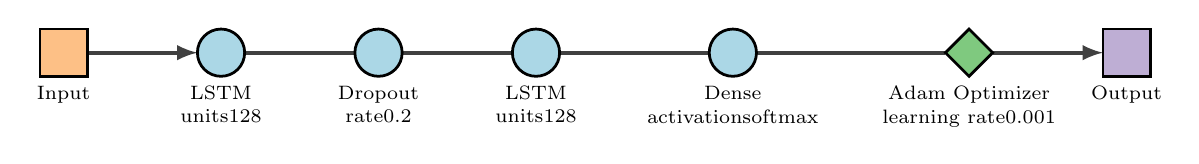
\begin{tikzpicture}
\Vertex[x=1,position=below,label=Input,RGB,color={253,192,134},shape=rectangle]{input}
\Vertex[x=3,position=below,label=LSTM]{lstm0}
\Vertex[x=3,position=below,label=units\eq 128,Pseudo,distance=3mm]{lstm0_}
\Vertex[x=5,position=below,label=Dropout]{dropout}
\Vertex[x=5,position=below,label=rate\eq 0.2,Pseudo,distance=3mm]{dropout_}
\Vertex[x=7,position=below,label=LSTM]{lstm1}
\Vertex[x=7,position=below,label=units\eq 128,Pseudo,distance=3mm]{lstm1_}
\Vertex[x=9.5,position=below,label=Dense]{dense}
\Vertex[x=9.5,position=below,label=activation\eq softmax,Pseudo,distance=3mm]{dense_}
\Vertex[x=12.5,position=below,label=Adam Optimizer,RGB,color={127,201,127},shape=diamond]{adam}
\Vertex[x=12.5,position=below,position=below,label=learning rate\eq 0.001,Pseudo,distance=3mm]{adam_}
\Vertex[x=14.5,position=below,label=Output,RGB,color={190,174,212},shape=rectangle]{output}
\Edge[Direct](input)(lstm0)
\Edge(lstm0)(dropout)
\Edge(dropout)(lstm1)
\Edge(lstm1)(dense)
\Edge(dense)(adam)
\Edge[Direct](adam)(output)
\end{tikzpicture}
\end{center}
\end{figure}

\subsection{验证}\label{sec:validation}

\begin{wraptable}{R}{6cm}
%\vspace{-50pt}
\caption{不同算法准确率对比} \label{tab:acc}
\begin{tabular}{ c | r | r }
\hline
           &   情绪 &           基调 \\ \hline
K-近邻算法 & 26.8\% & (未进行训练) \\ \hline
支持向量机 & 28.4\% & (未进行训练) \\ \hline
 LSTM 算法 & 75.4\% &         85.5\% \\ \hline
\end{tabular}
\vspace{-10pt}
\end{wraptable}

经过训练和测试,三种算法对音乐特征进行识别的准确率如表~\ref{tab:acc}~所示。这些准确率都是在验证集而非训练集上产生的。

其中对于 LSTM,我们进一步进行了混淆矩阵的计算,结果如表~\ref{tab:moodcm}、表~\ref{tab:genrecm}~所示。表中的百分比指的是某一种情况的数据占总数据的比,如“实际:sad 预测:calm 数据:1.2\%”指数据集中标签为 sad 而算法给出的预测结果为 calm 的音乐占总验证集音乐数量的 1.2\%。从表中的数据我们可以看出,算法给出的结果与真实结果相差较大的地方都是区分较为模糊的地方(例如 calm 和 sad),表明算法实现较好。

\begin{center}
% 请不要编辑下面的两个表格,谢谢!

\captionof{table}{情绪混淆矩阵(出于空间限制,部分情感只显示前面一部分字符,下同)} \label{tab:moodcm}
\begin{tabular}{ | r r | r | r | r | r | r | r | r | r | r | r | }
\hline
 & \bf 预测 & \bf calm & \bf dark & \bf sad & \bf drama & \bf funky & \bf happy & \bf bright & \bf roman & \bf inspi & \bf angry \\
\bf 实际 & & 17.0\% & 14.1\% & 1.0\% & 20.7\% & 9.4\% & 21.1\% & 10.7\% & 0.2\% & 3.5\% & 2.3\% \\\hline
\bf calm & 14.3\% & 11.7\% & 0.6\% & 0.0\% & 0.4\% & 0.0\% & 0.6\% & 0.6\% & 0.0\% & 0.4\% & 0.0\% \\\hline
\bf dark & 12.7\% & 0.4\% & 10.9\% & 0.0\% & 0.6\% & 0.4\% & 0.2\% & 0.0\% & 0.0\% & 0.0\% & 0.2\% \\\hline
\bf sad & 3.3\% & 1.2\% & 0.2\% & 1.0\% & 0.2\% & 0.0\% & 0.2\% & 0.6\% & 0.0\% & 0.0\% & 0.0\% \\\hline
\bf drama & 18.0\% & 0.2\% & 0.2\% & 0.0\% & 15.8\% & 0.0\% & 0.6\% & 1.2\% & 0.0\% & 0.0\% & 0.0\% \\\hline
\bf funky & 11.5\% & 0.6\% & 1.2\% & 0.0\% & 0.4\% & 7.8\% & 1.4\% & 0.2\% & 0.0\% & 0.0\% & 0.0\% \\\hline
\bf happy & 17.2\% & 0.4\% & 0.2\% & 0.0\% & 0.4\% & 0.2\% & 15.6\% & 0.2\% & 0.0\% & 0.0\% & 0.2\% \\\hline
\bf bright & 10.4\% & 0.4\% & 0.4\% & 0.0\% & 0.8\% & 0.2\% & 1.2\% & 7.4\% & 0.0\% & 0.0\% & 0.0\% \\\hline
\bf roman & 2.7\% & 1.4\% & 0.2\% & 0.0\% & 0.4\% & 0.0\% & 0.2\% & 0.6\% & 0.0\% & 0.0\% & 0.0\% \\\hline
\bf inspi & 6.4\% & 0.8\% & 0.2\% & 0.0\% & 1.2\% & 0.4\% & 0.6\% & 0.0\% & 0.2\% & 3.1\% & 0.0\% \\\hline
\bf angry & 3.5\% & 0.0\% & 0.0\% & 0.0\% & 0.6\% & 0.4\% & 0.6\% & 0.0\% & 0.0\% & 0.0\% & 2.0\% \\\hline
\end{tabular}

\captionof{table}{基调混淆矩阵} \label{tab:genrecm}
\begin{tabular}{ | r r | r | r | r | r | r | r | r | r | r | }
\hline
 & \bf 预测 & \bf cine & \bf rock & \bf amb & \bf jazz & \bf dance & \bf pop & \bf r\&b & \bf child & \bf count \\
\bf 实际 & & 24.2\% & 13.3\% & 8.0\% & 3.3\% & 17.6\% & 18.8\% & 6.3\% & 1.2\% & 7.4\% \\\hline
\bf cine & 21.9\% & 20.3\% & 0.4\% & 0.0\% & 0.0\% & 0.4\% & 0.4\% & 0.0\% & 0.0\% & 0.4\% \\\hline
\bf rock & 12.3\% & 0.2\% & 11.5\% & 0.0\% & 0.0\% & 0.6\% & 0.0\% & 0.0\% & 0.0\% & 0.0\% \\\hline
\bf amb & 9.0\% & 1.2\% & 0.0\% & 7.4\% & 0.0\% & 0.2\% & 0.2\% & 0.0\% & 0.0\% & 0.0\% \\\hline
\bf jazz & 5.3\% & 0.4\% & 0.2\% & 0.0\% & 3.1\% & 1.0\% & 0.4\% & 0.0\% & 0.0\% & 0.2\% \\\hline
\bf dance & 16.0\% & 0.2\% & 0.2\% & 0.4\% & 0.0\% & 14.1\% & 1.2\% & 0.0\% & 0.0\% & 0.0\% \\\hline
\bf pop & 17.0\% & 0.6\% & 0.0\% & 0.0\% & 0.0\% & 0.8\% & 15.6\% & 0.0\% & 0.0\% & 0.0\% \\\hline
\bf r\&b & 7.8\% & 0.2\% & 0.4\% & 0.0\% & 0.0\% & 0.6\% & 0.4\% & 6.1\% & 0.0\% & 0.2\% \\\hline
\bf child & 3.1\% & 1.0\% & 0.0\% & 0.0\% & 0.2\% & 0.0\% & 0.4\% & 0.0\% & 1.2\% & 0.4\% \\\hline
\bf count & 7.6\% & 0.2\% & 0.6\% & 0.2\% & 0.0\% & 0.0\% & 0.2\% & 0.2\% & 0.0\% & 6.3\% \\\hline
\end{tabular}

\end{center}

经过最终的调试,我们选择了准确率较高的 LSTM 算法,并进行程序封装。

\subsection{预测}\label{sec:predict}

对于需要预测的每首音乐,我们需要先进行音乐特征提取和数据正则化。进行完这些后,将数据输入图~\ref{fig:net}~所示的网络中,对网络的输出取 argmax,在对应表中找到数字对应的标签,即可得到预测的情感和基调。

\section{成果与展望}

\subsection{程序封装}

我们将智能配乐分类系统封装为了网页程序,用户可以通过上传音乐来创建自己的曲库,上传成功后,系统会自动排队解析;
解析成功后程序会以列表形式展示各配乐的参数,用户可以通过在在搜索栏输入限制条件(见代码~\ref{lst:search})来查找自己需要的配乐,程序会在曲库中筛选,并列出符合用户需求的音乐;
用户可以通过点击配乐名称来查看单首配乐的详细信息,包含长度、情感、乐器等参数和音乐波形图(并展示停顿、节拍等信息,见图~\ref{fig:wave}),用户还可以通过编辑功能来矫正自己认为识别不够准确的标签。
我们使用这一系统拍摄了一个演示视频,见~\url{https://www.bilibili.com/video/av625750106}。

\subsection{未来的完善方向}

\newcommand{\skpv}{\vspace{-10pt}}
\paragraph{分类乐器} 由于本研究数据源中乐器标签过于混乱,乐器识别功能基本不可用。后续可以找到更好的数据源进行识别;
\skpv\paragraph{尝试其他音乐特征} 尝试使用自相似矩阵等其他音乐特征,并增加到程序中;
\skpv\paragraph{尝试其他神经网络} 使用其他神经网络进行实验,找到更适合的算法,以进一步提升程序对音乐特征(情绪、乐器等)识别的准确率;
\skpv\paragraph{增加用户反馈模块} 增加用户反馈模块用于完善模型,用户在每次使用后可以在系统中对所用音乐的分类准确度进行评价,包括情绪、乐器、节奏识别的准确程度、程序使用体验等,用户在提交评价还可以选择将自己的音乐反馈给项目组作为训练,并附加自己认为正确的标签。用户也可以选择在矫正自己认为识别不够准确的标签后将音乐盒相关数据提交给项目组;
\skpv\paragraph{自动推荐配乐} 通过接入的用户登录,记录用户行为,在后期实现程序可以自动根据用户平时挑选音乐的风格偏好在首页智能推荐用户可能需要的配乐。

\section{团队分工}

梁亚伦负责研究计划的制定、训练数据的获取及预处理、训练程序的设计及实现、结果评价、程序封装的设计及实现,以及论文的撰写;
吴轩南负责问题的提出及研究目标的确定、研究计划的制定、前期调研、音乐分类体系的建立、交互界面的设计、展示短片的制作,以及论文的撰写;
李信义负责研究计划的制定、乐器标签的整理、算法的调研,以及论文的撰写。

\section{致谢}

在这一学年的学习和研究中,我们收获颇多。
首先,要特别感谢在过程中给予我们指导和监督的武迪老师与卢婧华老师,老师们在选题指导、思路启发等方面提出了很多宝贵的意见与建议。
由于疫情原因后半部分的研学课程不能正常在学校开展,老师们通过线上会议的方式有针对性的督促我们高效的完成研学任务,
还为我们邀请了来自业界领先企业的专家进行点评指导。同时,还要感谢团队成员间的戮力合作和沟通磨合,以及课程助教余锴诚学长的诸多帮助。
更要感谢参考文献和自由软件的作者们~\cite{tf15}\cite{CC01a}\cite{lstm15}\cite{boixx14}\cite{librosa18}\cite{lstm18},
他们的文章和研究成果为我们的项目提供了极大参考和帮助,在此也向他们表示感谢。

\bibliography{paper}{}
\bibliographystyle{plain}

\appendix

\section{代码}

\captionof{listing}{music.py} \label{lst:music}
\begin{minted}{python}
# 提取MFCC
self.mfcc = librosa.feature.mfcc(y=self.y, sr=self.sr)
# 提取Onset
self.onset_envelope = librosa.onset.onset_strength(y=self.y, sr=self.sr)
self.onset_frames = librosa.onset.onset_detect(onset_envelope=self.onset_envelope, sr=self.sr)
# 提取Beat
self.tempo, self.beats = librosa.beat.beat_track(onset_envelope=self.onset_envelope, sr=self.sr)
# 提取自相似矩阵
self.recurrence_matrix = librosa.segment.recurrence_matrix(self.mfcc)
# 提取Chroma
self.chroma = librosa.feature.chroma_stft(y=self.y, sr=self.sr)
# 提取viterbi
rms = librosa.feature.rms(y=self.y)[0]
r_normalized = (rms - 0.02) / np.std(rms)
p = np.exp(r_normalized) / (1 + np.exp(r_normalized))
self.viterbi = librosa.sequence.viterbi_discriminative(
  np.vstack([1 - p, p]), librosa.sequence.transition_loop(2, [0.5, 0.6]))
\end{minted}

\captionof{listing}{train.js} \label{lst:train}
\begin{minted}{javascript}
// 定义模型
const model = sequential()
model.add(lstm({ units, inputShape, returnSequences: true })) // LSTM, units = 128
model.add(dropout(0.2))                                       // Dropout
model.add(lstm({ units, returnSequences: true }))             // LSTM
model.add(dense({ units: nClasses, activation: 'softmax' }))  // Softmax

// 运行模型
;(async () => {
  // 如果是之前训练到一半接着训练的把下面一行取消注释,把上面一段注释掉
  // const model = await loadLayersModel('file://./model-30/model.json')

  // 定义训练方法
  model.compile({
    loss: 'categoricalCrossentropy', // 交叉熵
    optimizer: adam(learningRate),
    metrics: [ 'acc' ],
  })
  // 进行训练
  await model.fitDataset(
    dataset.batch(batchSize, false),
    { epochs, callbacks: {
      // 中途保存训练数据
      onEpochEnd(epoch) {
        if (epoch % 10 === 0) model.save(savePath + epoch)
      },
    } }
  )
  await model.save(savePath)
})().catch(e => {
  // 捕获训练中的异常并报错
  console.error(e && e.stack || e)
  process.exit(1)
})
\end{minted}

\captionof{listing}{搜索示例} \label{lst:search}
\paragraph{示例搜索文本} \texttt{piano, dur in 80-100 / (duration in 10-20, calm), tempo around 120, no pause-time > 10, stop <= 5, not time in 90 - 120}
\paragraph{含义} 找出标签含有 \texttt{piano},并且要么长度在 80 到 100 秒之间,要么长度在 10 到 20 秒之间并且情感是 \texttt{calm};并且节拍大约为 120 bpm,并且没有大于 10 秒的停顿,并且停顿数量少于 5 处,并且长度不在 90 到 120 秒之间的音乐。
\paragraph{对应代码}
\begin{minted}{javascript}
const predicate = music =>
  (music.tags.includes('piano') || music.mood === 'piano' || music.genre === 'piano') &&
  (
    (music.duration >= 80 && music.duration <= 100) ||
    (
      music.duration >= 10 && music.duration <= 20 &&
      (music.tags.includes('calm') || music.mood === 'calm' || music.genre === 'calm')
    )
  ) &&
  music.tempo >= 104 && music.tempo <= 136 &&
  !music.pauses.some(pause => pause > 10) &&
  music.pauses.length <= 5 &&
  !(music.time >= 90 && music.time <= 120)
\end{minted}

\end{document}
